\section{Siamese Multi-Object Tracking and Attention}
\label{sec:SiamMOTandAttention}

% ##############################################################################
\subsection{Motivation}

During several evaluation runs and our manual inspection of the tracker performance, we noticed a ubiquitous pattern. We remind that the scenes on which we trained as well as tested our tracker were captured by a static camera. Consequently, several video sequences contained multiple vehicles standing still, due to a traffic jam or an ongoing red light, but viewed under an angle somewhere in the range of $30-60$ degrees (see
\figtext{}~\ref{fig:UADETRACPartialOcclusion}). Therefore, it resulted in a partial occlusion. However, what we considered even more problematic was the inability of the axis-aligned \gls{bbox} to properly define the vehicle as the angle under which the car was visible caused the \gls{bbox} to capture a great portion of the neighboring vehicles even without severe occlusion happening.

% ------------------------------------------------------------------------------
\begin{figure}[!t]
    \centerline{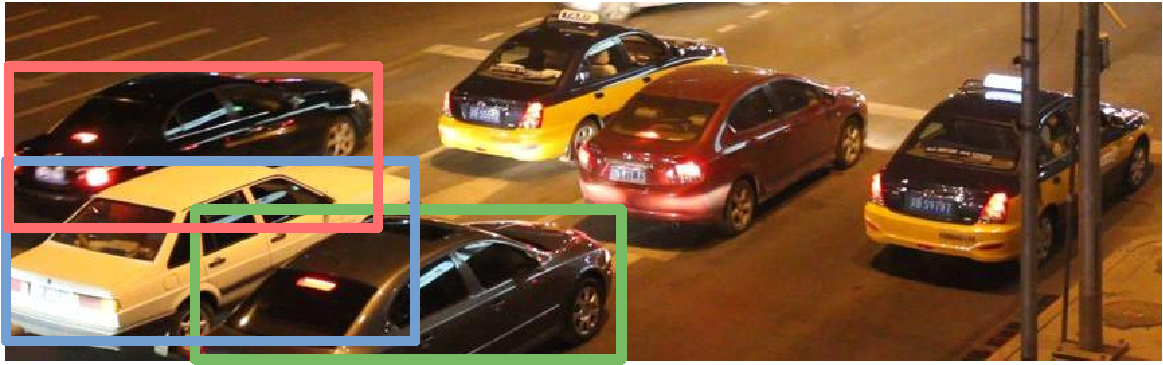
\includegraphics[width=0.7\linewidth]{figures/siamese_tracking/uadetrac_partial_occlusion_red_light.pdf}}
    \caption[Partial occlusion in the \uadetrac{} dataset]{An example of a situation where multiple vehicles are standing still on a cross-road. In this scenario, even though a slight degree of occlusion is necessary, the biggest issues are caused by the need to delineate \glspl{roi} using axis-aligned \glspl{bbox}. This inevitably captures the neighboring vehicles, increasing the likelihood of drifting to semantic background due to presence of similar interference, \ietext{}, distractors.}
    \label{fig:UADETRACPartialOcclusion}
\end{figure}
% ------------------------------------------------------------------------------

Situations described above reminded us of the \gls{siammask}~\cite{wang2019siammask} single object tracker targeted at predicting segmentation mask along with the usual single-object Siamese tracking routine. Such prediction was subsequently exploited to produce a rotated \gls{bbox} instead of an axis-aligned one. Even though the evaluation benchmarks only consider axis-aligned predictions, the rotated region served the purpose of enhancing the discriminative power of the tracker, primarily when dealing with occlusion. In the scenario shown in \figtext{}~\ref{fig:UADETRACPartialOcclusion}, a rotated \gls{bbox} would inexorably lead to an improved tracking accuracy. This approach was deemed successful for general object tracking, thus it also spawned another follow-up work of \gls{siammaske}~\cite{chen2019rotbboxes} which altered the original formulation of predicting the rotated \gls{bbox} by use of ellipse fitting for even better accuracy.

However, as stated by the authors as well, there is a lack of datasets providing rotated annotations. The \uadetrac{} dataset is no exception. As a result, we sidestepped this approach and searched for an alternative solution that would enhance the discriminative power of the tracker when faced with partial occlusion. One such approach was the use of attention~\cite{vaswani2017attention}, especially spatial attention, which we found effective during our survey research~\cite{ondrasovic2021siamese}. Apart from the attention mechanism, we also remembered the more general formulation of the convolution operation, which has been shown to significantly better object detection tasks due to the semi-dense prediction requirements, dubbed as deformable convolution~\cite{dai2017dcnn}. In what follows, we shall discuss these two methods (\sectiontext{}~\ref{ssec:Attention} and \sectiontext{}~\ref{ssec:DeformableCNNs}) as a foundation for our subsequent experiments that yielded a positive outcome.

% ##############################################################################
\subsection{Attention}
\label{ssec:Attention}

An attention mechanism was first introduced by Vaswani~\etal{}~\cite{vaswani2017attention}. The use of encoder-decoder architectures to capture a complete sequence of information by a single vector spurred the development of the attention module. This use case poses problems in holding on to information at the beginning of the sequence and encoding long-range dependencies. To address this, the attention module computes attentions, or, in other words, the degree of relevance between ``queries'' and ``keys'', to retrieve ``values'' in adequate proportions.

The concept of ``queries, keys and values'' comes from information retrieval systems. Let us provide a demonstrative example based on a YouTube video search. Assume a specific query signaling the demand to retrieve a particular YouTube video. The system will then map this query against a set of keys represented by various features, \egtext{}, video title, description, upload time, etc. These keys are directly associated with the stored candidate videos within the database. The output of this operation is a set of values, \ietext{}, found videos, that best match the given query.

In abstract terms, attention aims to exploit deep learning to learn a transformation of the input (not necessarily the same) into three separate vector spaces, each of them dedicated to a different purpose. The first space is to capture the query, therefore, it should represent features that best describe the query to facilitate information retrieval. The obvious compatriot is the key vector space which is trained to represent the value in the most accurate way to initiate the search accurately. Last but not least, the value vector space extracts features that are most useful for the task at hand. They do not need to capture features pertinent to the search. For that, there are two other mappings.

For a more concrete demonstration, we shall use a scaled dot-product attention. The input consists of queries and keys of dimension $d_k$, and values of dimension $d_v$. The query is used to compute a dot product with all the keys. These computations are scaled by $\sqrt{d_k}$ to provide a temperature scaling for the following softmax transformation to obtain the weights that will be used to retrieve values (see \figtext{}~\ref{fig:ScaledDotProductAttention}). For optimal performance, it is reasonable to compute the attention function for the set of queries simultaneously as they can be easily stored in a matrix, denoted by $\mtx{Q}$. Analogically, keys and values can be also packed together into matrices given by $\mtx{K}$ and $\mtx{V}$, respectively. Thus, the attention can be formulated as a function of queries, keys and values, and is defined as
\begin{equation}
    \label{eq:ScaledDotProductAttention}
    \func{attention}{\mtx{Q}, \mtx{K}, \mtx{V}} =
    \func{softmax}{\frac{\mtx{Q} \mtx{K}^T}{\sqrt{d_k}}} \mtx{V}.
\end{equation}

% ------------------------------------------------------------------------------
\begin{figure}[!t]
    \centerline{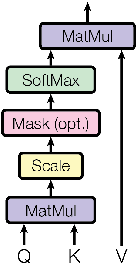
\includegraphics[width=0.15\linewidth]{figures/siamese_tracking/scaled_dot_product_attention.pdf}}
    \caption[Scaled dot-product attention]{An example of the input transformation by the scaled dot-product attention module. The pair of queries and keys is used to produce the probability distribution over the individual values for the final weighted sum. \externalsrc{\cite{vaswani2017attention}}}
    \label{fig:ScaledDotProductAttention}
\end{figure}
% ------------------------------------------------------------------------------

The two most prominent variants of attention are the additive attention~\cite{bahdanau2016additiveattention} and the multiplicative (dot-product) attention, with the latter being identical to the one described above except for the temperature scaling. Just for the record, we experimented with both approaches and we observed differences in performance. On balance, both attentions are similar in theory, however, dot-product is much faster and more space-efficient in practice. On the other hand, additive attention outperforms the dot-product attention as long as temperature scaling is not employed for larger values of $d_k$, since the dot-products tend to push the softmax function to regions of extremely small gradients.

In our work, we also exploited the notion of self-attention. Since attention was first targeted at natural language translation, let us provide an example from this area. Originally, the attention was computed between the input and output sentences. Regarding self-attention, attention is computed with respect to the sentence itself. In terms of computer vision, the spatial self-attention represents a weight map over a $2$D feature map indicating how important each feature element for the particular task is. Analogically, the channel self-attention may be used to attribute importance to individual channels, as they often are not equally important. Moreover, it yields more interpretable models as a by-product~\cite{vaswani2017attention}. These ideas will be explored later.

% ##############################################################################
\subsection{Deformable Convolutional Neural Networks}
\label{ssec:DeformableCNNs}

\Glspl{dcnn}~\cite{dai2017dcnn} are gaining popularity and are being applied to numerous sophisticated computer vision tasks, \egtext{}, object segmentation (dense predictions) and object detection (semi-dense predictions). Since object tracking revolves around the same requirements in terms of pixel-wise precision, we contemplated using this advancement, too.

Although \glspl{cnn} (\sectiontext{}~\ref{ssec:ConvolutionalNeuralNetworks} on page~\pageref{ssec:ConvolutionalNeuralNetworks}) are an excellent tool for a plethora of deep learning tasks involving image processing, they are still limited in their capabilities to model a broad range geometric transformation. To address this, practitioners apply a broad range of data augmentation techniques (\egtext{}, rotation, translation, scaling, shearing, and cropping) to provide the necessary samples of some particular transformation during the training. However, such an approach is limited to tailor-made transformations that may not cover the entire set of possibilities the model may face in practice.

The first work to learn spatial transformation from the training data in a deep learning fashion is known under the name \glspl{stn}~\cite{jaderberg2016stn}. It warps the feature map via a global parametric transformation such as affine transformation. In the real of convolutional operations, there is the atrous convolution operation~\cite{holschneider1990atrousconv} that enhances the standard convolution by expanding the receptive field while maintaining the same number of parameters by use of greater offsets. However, these offsets are fixed. An obvious successor of this approach is the active convolution~\cite{jeon2017activeconv} that treats convolution offsets as learnable parameters instead of constants. But, in this setting, the learned offsets are shared across different spatial locations. Thus, the most general approach is to determine the offsets at each location independently and then proceed as usual. This is where deformable convolution (see \figtext{}~\ref{fig:StandardVsDeformableCNN}) comes into place, discussed next.

In concrete terms, a $2$D convolution consists of sampling using a regular offset grid $\mset{R}$ defining the receptive field as well as dilation over the input features $\vect{x}$ followed by the summation of the samples values weighted by $\vect{w}$. For example, a standard $3 \times 3$ convolution with dilation $1$ would employ offsets given by
\begin{equation}
    \label{eq:StandardConvolutionOffsetGrid}
    \mset{R} = \cbrackets{
        \rbrackets{-1, -1}, \rbrackets{-1, 0}, \dots, \rbrackets{0, 1}, \rbrackets{1, 1}
    }.
\end{equation}
Then, for each location $\vect{p}_0$ within the output feature map $\vect{y}$ is calculated as
\begin{equation}
    \label{eq:StandardConvolutionOutputCalc}
    \func{\vect{y}}{\vect{p}_0} =
    \sum_{\forall \vect{p}_n \in \mset{R}}
    \func{\vect{w}}{\vect{p}_n} \cdot \func{\vect{x}}{\vect{p}_0 + \vect{p}_n},
\end{equation}
where the locations in $\mset{R}$ are iterated over by $\vect{p}_n$.

Conversely, the deformable convolution extends the standard one by augmenting the original sampling grid $\mset{R}$ with additional offsets $\cbrackets{\Delta \vect{p}_n \ |\ n = 1, \dots, \msetsize{R}}$ (see \figtext{}~\ref{fig:DeformableCNN}). Thus, \eqtext{}~\ref{eq:StandardConvolutionOutputCalc} is reformulated as
\begin{equation}
    \label{eq:DeformableConvolutionOutputCalc}
    \func{\vect{y}}{\vect{p}_0} =
    \sum_{\forall \vect{p}_n \in \mset{R}}
    \func{\vect{w}}{\vect{p}_n} \cdot \func{\vect{x}}{\vect{p}_0 + \vect{p}_n + \Delta \vect{p}_n}.
\end{equation}
However, one needs to keep in mind that the sampling offsets now become fractions and thus have to be handled accordingly. One approach is to employ bilinear interpolation, where the position in the input feature map $\vect{x}$ is determined by
\begin{equation}
    \label{eq:DeformableConvolutionBilinear}
    \func{\vect{x}}{\vect{p}} =
    \sum_{\forall \vect{q}} \func{G}{\vect{q}, \vect{p}} \cdot \func{\vect{x}}{\vect{p}},
\end{equation}
in which $\vect{q}$ enumerates all integral locations and $\func{G}{\cdot}$ represents the  interpolation kernel. The interpolation processing can be efficiently implemented owing to the sparsity. The performance overhead is negligible compared to the reaped benefits of adaptive sampling locations capable of covering very complicated transformations (see \figtext{}~\ref{fig:SamplingLocationsDeformableCNN}).

% ------------------------------------------------------------------------------
\begin{figure}[t]
    \centerline{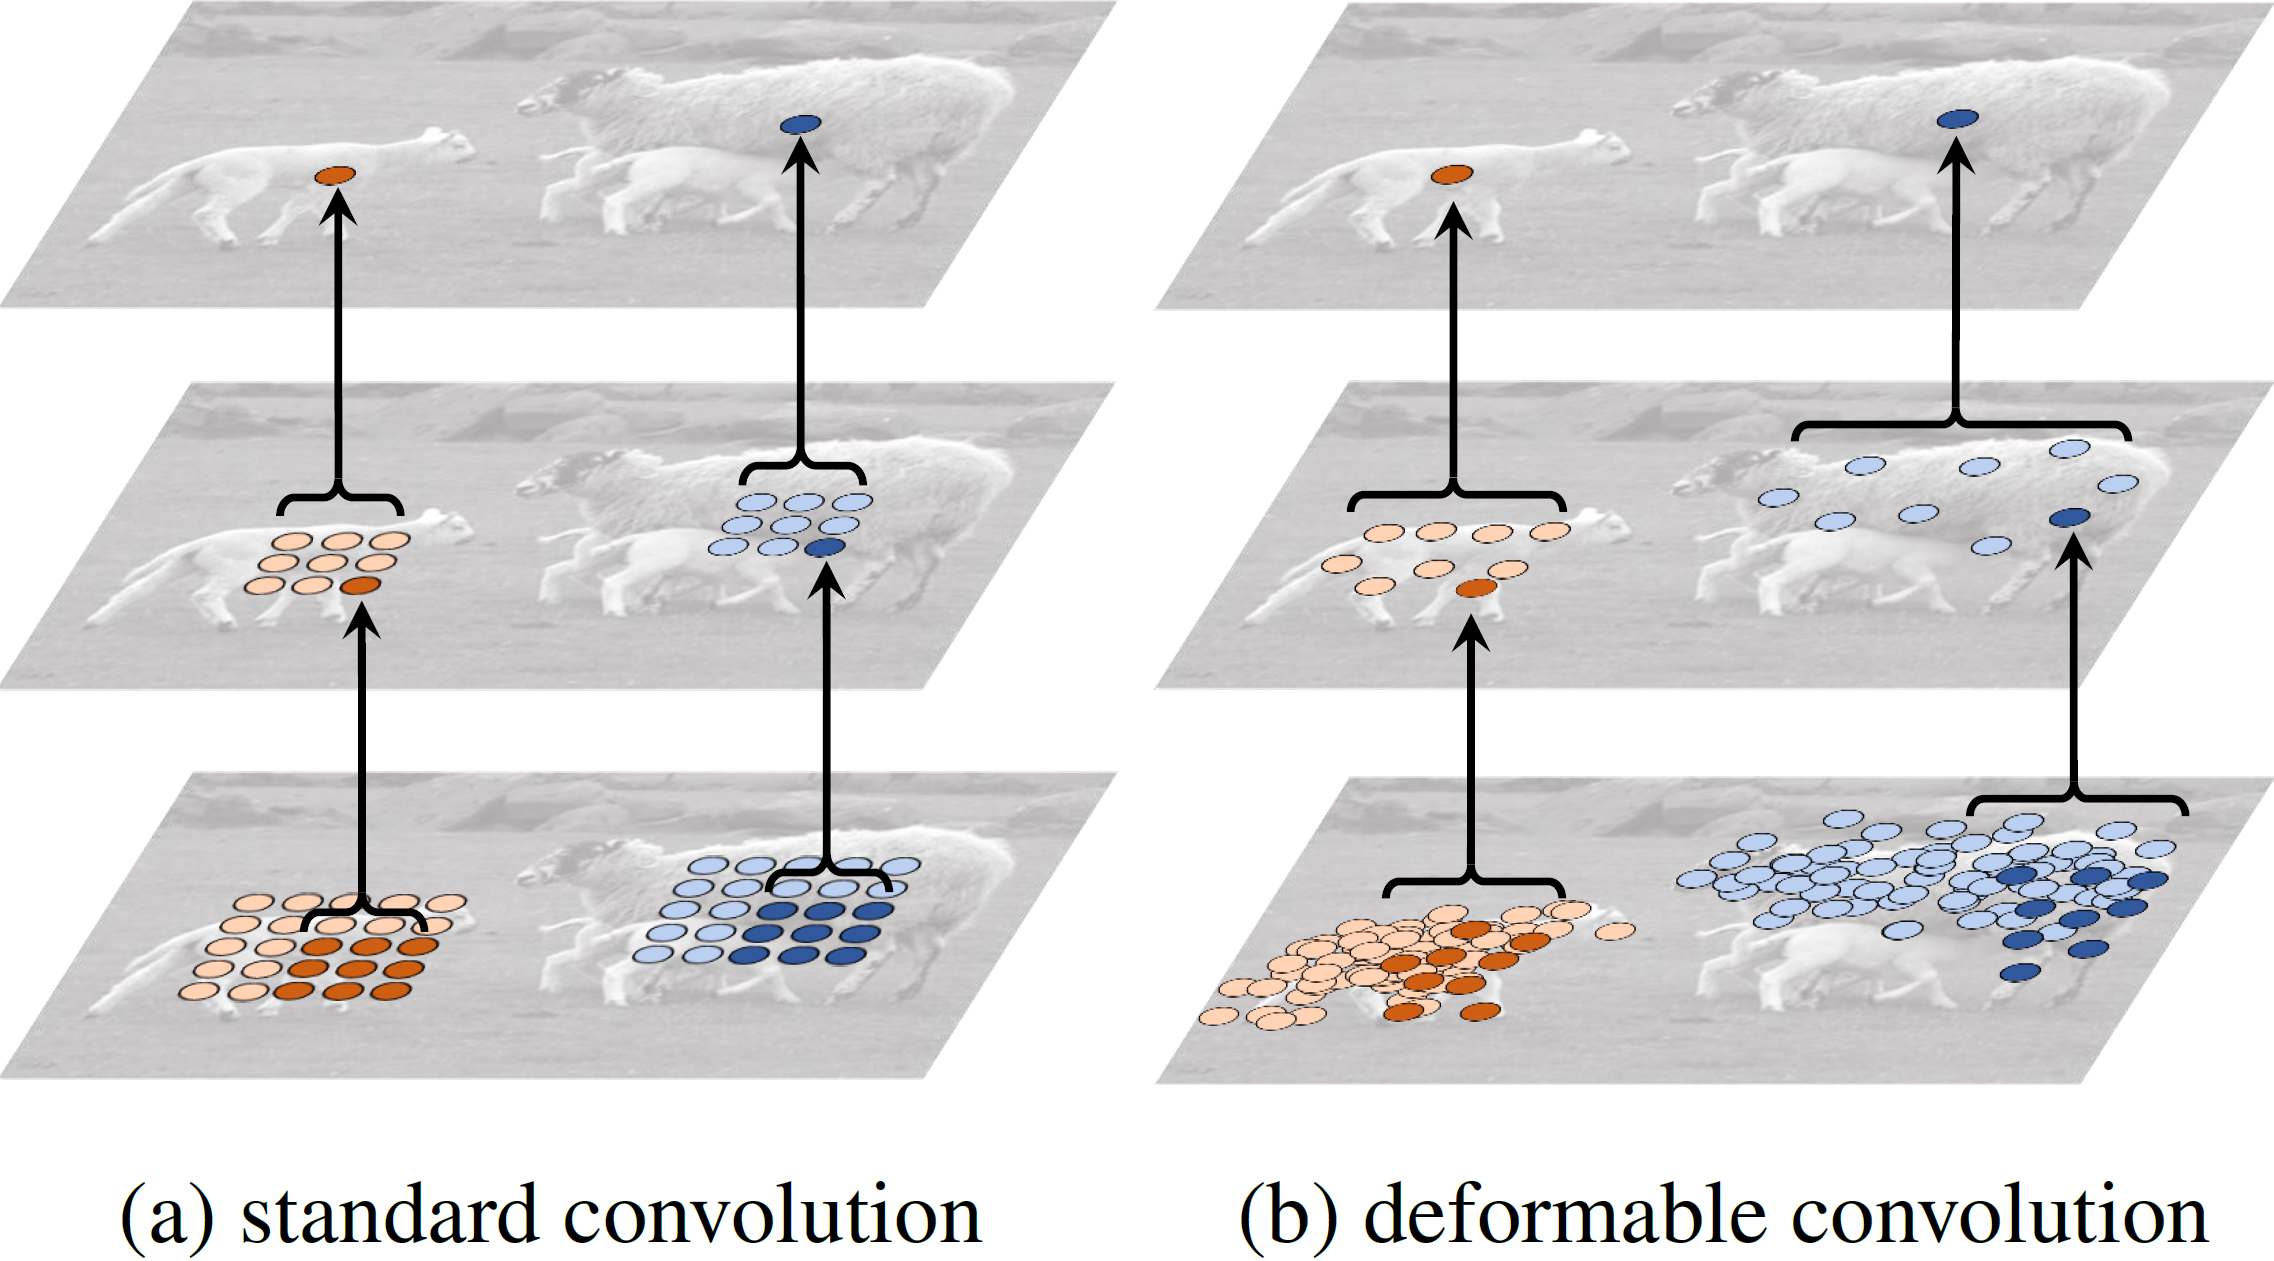
\includegraphics[width=0.6\linewidth]{figures/siamese_tracking/dcn_standard_vs_deformable.png}}
    \caption[Standard vs. deformable convolution]{Visualization of the difference between the fixed \imgpartdesc{a} and adaptive \imgpartdesc{b} receptive fields. Stacking multiple deformable convolutions results in profound amplification of deformation, making the transformation capture diverse shapes that would otherwise be very coarsely approximated by a standard convolution. \externalsrc{\cite{dai2017dcnn}}}
    \label{fig:StandardVsDeformableCNN}
\end{figure}
% ------------------------------------------------------------------------------

% ------------------------------------------------------------------------------
\begin{figure}[t]
    \centerline{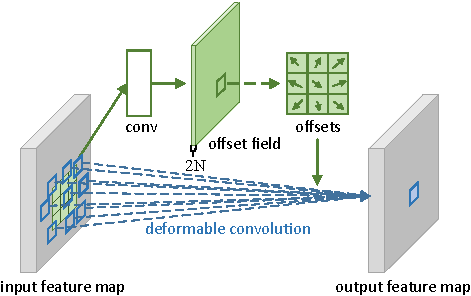
\includegraphics[width=0.5\linewidth]{figures/siamese_tracking/deformable_convolution.pdf}}
    \caption[\Gls{dcnn}]{Illustration of a $3 \times 3$ deformable convolution operation. Unlike the standard convolution operation used in neural networks, this one employs one additional step of predicting variable offsets instead of using a fixed rectangular grid. \externalsrc{\cite{dai2017dcnn}}}
    \label{fig:DeformableCNN}
\end{figure}
% ------------------------------------------------------------------------------

% ------------------------------------------------------------------------------
\begin{figure}[t]
    \centerline{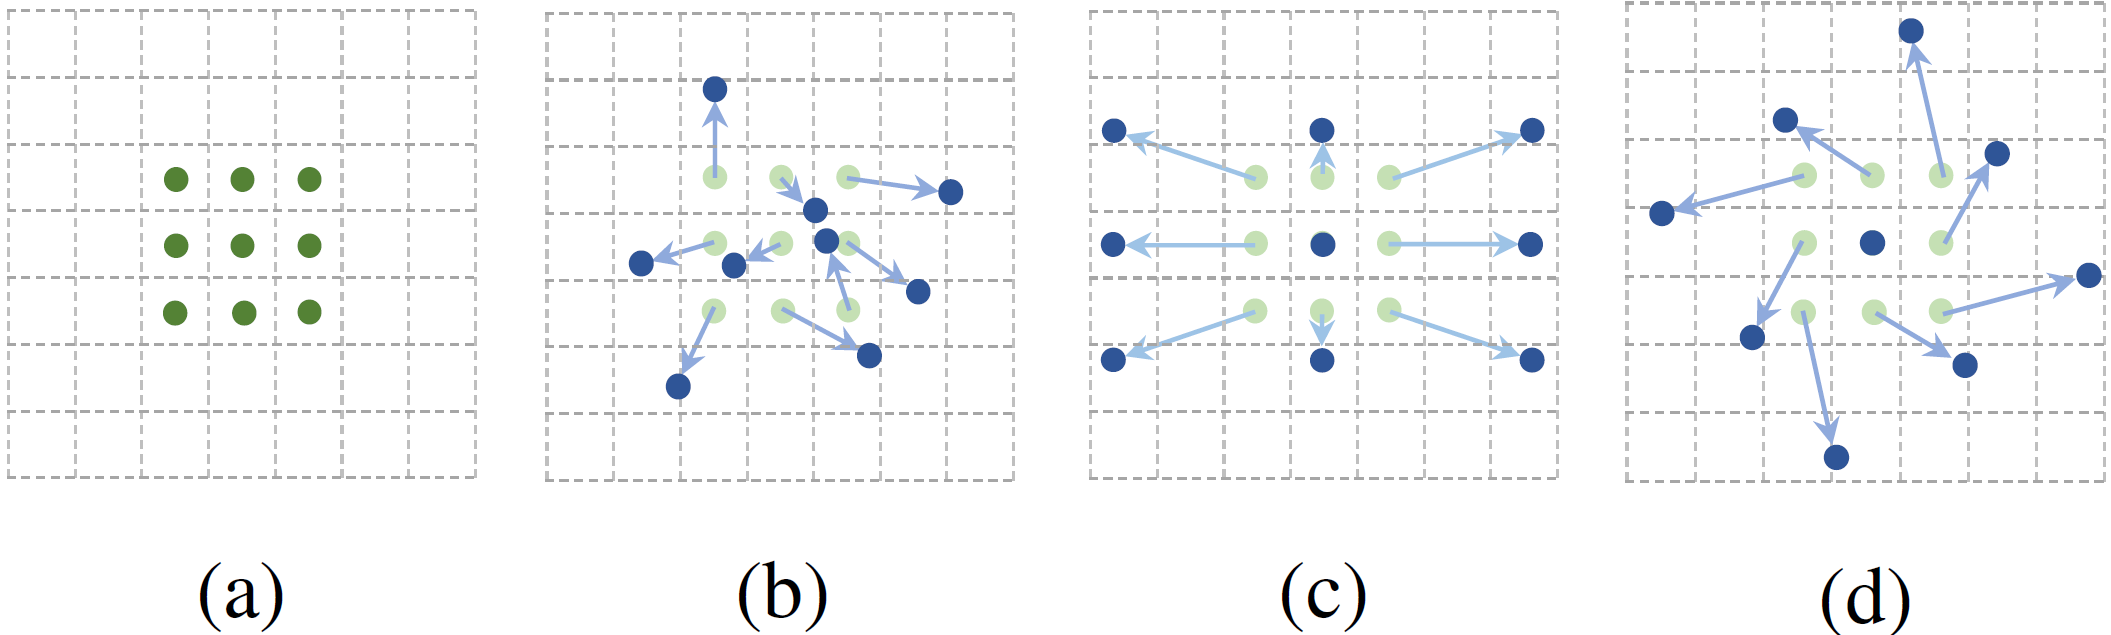
\includegraphics[width=0.7\linewidth]{figures/siamese_tracking/dcn_sampling_locations.png}}
    \caption[Various sampling locations in \glspl{dcnn}]{Deformable convolution is effective at learning appropriate sampling locations reflecting the underlying transformation. \imgpartdesc{a} shows the regular sampling grid of a standard convolution; \imgpartdesc{b} is an example of irregularly deformed sampling region; \imgpartdesc{c} and \imgpartdesc{d} represent an expected pattern corresponding to scaling and rotation operations, respectively. \externalsrc{\cite{dai2017dcnn}}}
    \label{fig:SamplingLocationsDeformableCNN}
\end{figure}
% ------------------------------------------------------------------------------

The original paper~\cite{dai2017dcnn}, where \glspl{dcnn} were introduced showed, that learning dense spatial transformation in using deep learning by use of \glspl{cnn} or sophisticated vision tasks such as object detection and semantic segmentation is feasible as well as effective. After our experience, we add that object tracking may benefit from this extension, too.

\subsection{Modulated Deformable Convolutional Neural Networks}
\label{ssec:ModulatedDeformableCNNs}

The original paper by Zhu~\etal{}~\cite{zhu2018mdcnn} aptly described their contribution in the headline that contained the words ``mode deformable, better results''. Because of this, we shall provide a concise description of the \glspl{mdcnn}, an extension to the previously discussed \glspl{dcnn}.

Since we are simply adding a slight modifications to an already introduced equation, we will try to avoid repetition. Thus, let $\vect{p}_0$, $\vect{p}_n$ and $\Delta \vect{p}_n$ have the same meaning as in \eqtext{}~\ref{eq:DeformableConvolutionOutputCalc}. Then, the modified equation becomes
\begin{equation}
    \label{eq:ModulatedDeformableConvolutionOutputCalc}
    \func{\vect{y}}{\vect{p}_0} =
    \sum_{\forall \vect{p}_n \in \mset{R}}
    \func{\vect{w}}{\vect{p}_n} \cdot \func{\vect{x}}{\vect{p}_0 + \vect{p}_n + \Delta \vect{p}_n} \cdot \Delta \vect{m}_n,
\end{equation}
where $\Delta \vect{m}_n$ is the modulation scalar for the current location, such that $\Delta \vect{m}_n \in \rbrackets{0, 1}$. Thus, there are two learnable parameters. The already described offsets, given by the $\Delta \vect{p}_n$ term, and the new modulation (weighting) coefficients, represented by the term $\Delta \vect{m}_n$.

This trivial extension allows the system to not only learn how to sample features in a non-regular fashion if needed, but it also allows applying distinct weight to each sampling location to further adaptively intensify the deforming effect.

From an implementation standpoint, \glspl{dcnn} as well as \glspl{mdcnn} have learnable offsets (and modulation coefficients, if used) set to zero during initialization. This produces no deformable effect, so the convolution behaves as usual in terms of location sampling. However, the modulation aspect is slightly different. Since the sigmoid function is commonly adopted to project the modulation weights into the $\rbrackets{0, 1}$ interval, it multiplies each location by the value of $\func{sigmoid}{0} = \nicefrac{1}{2}$ at the beginning.

% ##############################################################################
\subsection{Deformable Siamese Attention}
\label{ssec:DeformableSiameseAttention}

The two independent ideas above led us to experiment with a self-attention mechanism aimed at enhancing feature selection in both spatial and channel domains. Such experiments resulted in slight improvements for the reasons outlined in the motivation section. To support that our proposals were based on properly identified causes, we found a recently published work that demonstrated the effectiveness and potential use of our ideas, too.

Yu~\etal{}~\cite{yu2021dsa} formulated their \gls{dsa}, which covered both of our suggestions above and additionally introduced the notion of cross-attention as an enhancement to the self-attention itself. What primarily motivated the introduction of the cross-attention was that the exemplar and search region features in Siamese trackers are computed separately, yet they may frequently compensate each other. It is reasonable to assume that multiple objects appear at the same time even in \gls{sot}, let alone \gls{mot}. Consequently, it is of paramount importance for the search branch to have as much information as possible about the exemplar during the computation of the response map for better discrimination. By the same token, the exemplar features may be enhanced by information from the search features. To this end, the cross-attention, at the acceptable computational cost, serves well.

Considering their contribution and promising outcomes for the single object tracking demonstrated on the \gls{siamrpn} framework (first discussed in \sectiontext{}~\ref{ssec:TrackingUsingSiameseNetworks} on page \pageref{ssec:TrackingUsingSiameseNetworks}), we decided to implement their proposed module into the \gls{siammot} tracker as described in their paper. However, with the prospect of greater improvement, we adopted \glspl{dcnn}, instead of pure \glspl{dcnn}. The rationale behind this is the following. \Glspl{mdcnn} have all the advantages of the standard deformable convolution, but they additionally learn a modulation (weighting) for individual elements of the feature map while taking the underlying features into account. For our purposes, this seemed to intensify the spatial attention effect, since not only the deformable part was responsible for choosing features using irregular sampling patterns, the network was even allowed to weigh them differently. We conjectured that such an extension may either have no dramatic effect or influence it only positively.

% ------------------------------------------------------------------------------
\begin{figure}[t]
    \centerline{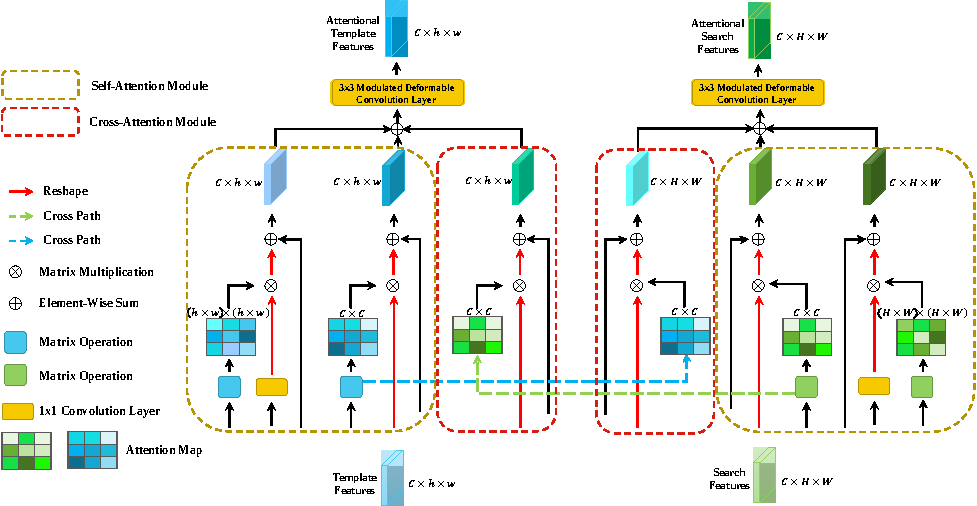
\includegraphics[width=\linewidth]{figures/siamese_tracking/deformable_siamese_attention.pdf}}
    \caption[\Gls{dsa} diagram]{The \gls{dsa} extension introduces two sub-modules for both exemplar and search branch. The self-attention is further divided into two operations, namely the spatial and channel attention. The very same attention network is used to process both features independently. Notice how the channel attention is computed only once as part of the self-attention process and then directly fused with the channel self-attention of the other branch, creating the cross-attention effect, which is the strongest one from all three, according to authors. In this figure, we modified the deformable convolution operation to include the modulated version, which is our modification compared to the original formulation. \externalsrc{\cite{yu2021dsa}}}
    \label{fig:DeformableSiameseAttention}
\end{figure}
% ------------------------------------------------------------------------------

\subsubsection{Self-Attention}

Self-attention is computed separately on the exemplar and search branch independently. This operation can be easily achieved since exemplar and search tensors only differ in width and height, which does not pose a problem to convolution at all (fully convolutional networks exploit this property). The following description of the self-attention computation conforms to the established attention principles regarding ``queries, keys and values'' introduced in \sectiontext{}~\ref{ssec:Attention}. For better understanding of the computation, see the diagram in \figtext{}~\ref{fig:DeformableSiameseAttention}.

Let $\mtx{X} \in \setrnnn{C}{H}{W}$ be the input features. To produce query features $\mtx{Q}$ and key features $\mtx{K}$, such that $\mtx{Q}, \mtx{K} \in \setrnnn{C^{\prime}} {H}{W}$ and $C^{\prime} = \frac{1}{4}C$, where $C^{\prime}$ is the reduced number of channels, first two separate $1 \times 1$ convolution layers are applied. The two obtained features then need to be reshaped into $\mtx{\bar{Q}}, \mtx{\bar{K}} \in \setrnn{C^{\prime}}{N}$, where $N = H \times W$. The spatial self-attention $\mtxsubsup{A}{S}{S} \in \setrnn{N}{N}$ is then produced via matrix multiplication and a column-wise softmax operation as
\begin{equation}
    \label{eq:SpatialSelfAttention}
    \mtxsubsup{A}{S}{S} =
    \func{softmax_{col}}{\mtx{\bar{Q}}^T \mtx{\bar{K}}}.
\end{equation}
Authors used $C^{\prime} = \frac{1}{8}C$, but in \gls{mot}, the number of objects to track is often a lot greater, thus the computation graph grows dramatically with the higher number of channels. Furthermore, in our case $C = 128$, and we considered using $32$ channels for the attention to be the bare minimum.

Meanwhile, an analogous sequence of operations is adopted to produce the value features. A $1 \times 1$ convolution layer without the subsequent reshape operation transforms the input features $\mtx{X}$ into the value features $\mtx{\bar{V}} \in \setrnn{C}{N}$. At this point, we have matched the queries and keys as well as computed the values. We may proceeed further to the weighted selection from the values and to incorporate the attention into the features as follows
\begin{equation}
    \label{eq:SpatialSelfAttentionApplication}
    \mtxsubsup{\bar{X}}{S}{S} =
    \alpha \mtx{\bar{V}} \mtxsubsup{A}{S}{S} + \mtx{\bar{X}},
\end{equation}
where $\alpha$ is a learnable scalar parameter, and $\mtxsubsup{\bar{X}}{S}{S} \in \setrnn{C}{N}$. The outputs $\mtxsubsup{\bar{X}}{S}{S}$ are then reshaped back to the original size, specifically $\mtxsubsup{X}{S}{S} \in \setrnnn{C}{H}{W}$. From our experience, the parameter $\alpha$ is very useful for training stabilization.

The corresponding channel self-attention $\mtxsubsup{A}{C}{S}$ and the channel-wise attentional features $\mtxsubsup{X}{C}{S}$ are obtained similarly. Due to space limitations and the fact that the upcoming formulation of the cross-attention exploits the channel self-attention, we will omit a detailed description. We will just point out that the ``queries, keys and values'' for the channel self-attention are produced directly from the features on the input, with no $1 \times 1$ convolutions whatsoever. The final self-attentional features are generated by an element-wise sum using the partial spatial and channel self-attentions, $\mtxsubsup{X}{S}{S}$ and $\mtxsubsup{X}{C}{S}$, respectively.

\subsubsection{Cross-Attention}

Let $\mtx{Z} \in \setrnnn{C}{h}{w}$, $\mtx{X} \in \setrnnn{C}{H}{W}$ denote the exemplar and search region features, respectively. The following description introduces the computation of the cross-attention from the perspective of the search branch. First, the exemplar features $\mtx{Z}$ are reshaped into $\mtx{\bar{Z}} \in \setrnn{C}{n}$, where $n = h \times w$. Then, the cross-attention from the exemplar branch is computed. We emphasize that the channel attention is reused, therefore, the computation below serves as a recipe for how to compute the channel self-attention. So, we compute the channel cross-attention $\mtxsup{A}{C} \in \setrnn{C}{C}$ as
\begin{equation}
    \label{eq:CrossAttentionCalc}
    \mtxsup{A}{C} =
    \func{softmax_{row}}{\mtx{\bar{Z}} \mtx{\bar{Z}}^T}.
\end{equation}
The real benefit comes from the merging stage, where the above-computed attention is merged with the other, in this case, the search branch as
\begin{equation}
    \label{eq:CrossAttentionMerge}
    \mtxsup{\bar{X}}{C} =
    \gamma \mtxsup{A}{C} \mtx{\bar{X}} + \mtx{\bar{X}},
\end{equation}
where $\gamma$ is a learnable scalar parameter. The merged features $\mtxsup{\bar{X}}{C}$, once again, have to be reshaped, so the features $\mtxsup{X}{C} \in \setrnnn{C}{H}{W}$ are the final output.

At last, the self-attentional features are combined with the cross-attentional features using element-wise sum. The cross-attention from the perspective of the exemplar branch can be obtained using a similar sequence of operations. In total, there are six steps that involve addition for the purpose of feature merging (see \figtext{}~\ref{fig:DeformableSiameseAttention}).

Once the attention is applied to tracking, the corresponding response map is altered as expected. Discriminative power of the tracker is enhanced by appropriate suppression of the semantic background. As \figtext{}~\ref{fig:DSAAttentionVisualization} shows, activations in the search regions as viewed through the response map vary if the \gls{dsa} module is included in the computation, making the tracker less prone to drifting to scene or semantic background objects.

\subsubsection{Deformable Convolution Phase}

The attention is finalized by processing the obtained feature tensors by another layer of deformable convolution, in our case, modulated deformable convolution. The resulting features the shape of which is identical to the input shape are used to compute the response map. As a result, this extension can be easily integrated into an existing pipeline thanks to its ability to preserve tensor shapes.

% ------------------------------------------------------------------------------
\begin{figure}[t]
    \centerline{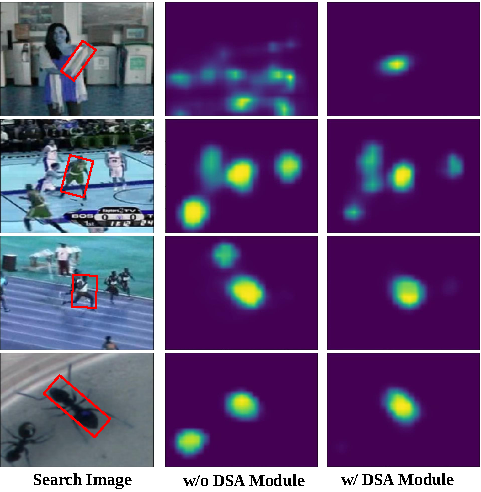
\includegraphics[width=0.5\linewidth]{figures/siamese_tracking/dsa_attention_visualization.pdf}}
    \caption[\Gls{dsa} attention visualization]{Visualization of response (confidence) maps. The first column represents the search image, the second column represents the activation levels without the \gls{dsa} module, whereas the third column clearly demonstrates the improved target-background discirminability in the computed attentional features. \externalsrc{\cite{yu2021dsa}}}
    \label{fig:DSAAttentionVisualization}
\end{figure}
% ------------------------------------------------------------------------------

% ##############################################################################
\subsection{Experimental Evaluation}
\label{ssec:DSAExperimentalEvaluation}

% ##############################################################################
\subsection{Discussion}
\label{ssec:DSADiscussion}
